% !TEX program = xelatex
% [EN] Reuse verified source crops and count PDF covers in page locators. / [CN] 复用已核验的原文截图，PDF 定位页码包含封面。
\documentclass[11pt,a4paper]{article}
\usepackage[margin=22mm,headheight=15pt]{geometry}
\usepackage{fontspec}
\setmainfont{TeX Gyre Termes}
\setsansfont{TeX Gyre Heros}
\usepackage{amsmath,amssymb,bm,graphicx,float,caption}
\usepackage{booktabs,tabularx,array,xcolor,fancyhdr,enumitem}
\usepackage[numbers,sort&compress]{natbib}
\usepackage{xurl}
\usepackage[colorlinks=true,linkcolor=blue!45!black,citecolor=blue!45!black,urlcolor=blue!45!black]{hyperref}
\graphicspath{{figures/}}
\setlength{\parindent}{0pt}
\setlength{\parskip}{5pt}
\setlength{\emergencystretch}{2em}
\captionsetup{font=small,labelfont=bf,justification=raggedright,singlelinecheck=false}
\setlist{nosep,leftmargin=1.5em}
\renewcommand{\arraystretch}{1.18}
\newcolumntype{Y}{>{\raggedright\arraybackslash}X}
\pagestyle{fancy}\fancyhf{}
\fancyhead[L]{\small\sffamily RIKEN polarized deuterons}
\fancyhead[R]{\small Production, transport and polarimetry}
\fancyfoot[C]{\thepage}
\newcommand{\src}[2]{~\cite[#2]{#1}}
\newcommand{\unit}[1]{\,\mathrm{#1}}
\newcommand{\shot}[4]{\begin{figure}[H]\centering\includegraphics[width=#2\linewidth]{#1}\caption{#3}\label{#4}\end{figure}}
\hypersetup{pdftitle={Polarized Deuterons at RIKEN: Production, Transport and Experimental Responsibilities},pdfauthor={Polarimeter project}}
\title{\sffamily Polarized Deuterons at RIKEN\\[3pt]\large Production, Transport and Experimental Responsibilities}
\author{Polarimeter project \quad | \quad Concise English edition}
\date{Sources checked: 7 September 2026}
\begin{document}
\maketitle\thispagestyle{empty}

\textbf{The experimental objective is a calibrated spin state at the reaction target.}
The polarized ion source prepares the spin populations and axis; the cyclotrons maintain a controlled spin phase; calibrated polarimeters establish the polarization along the beam path. For SAMURAI, these measurements feed a transport model that gives the target polarization for each source mode and time interval. The operational support to discuss with Sekiguchi's team covers PIS mode tuning, spin-axis setting, extraction diagnostics and polarization monitoring throughout the run.

\section{Production and beam delivery}
The established high-energy acceleration chain is
\[
\mathrm{PIS}\to\mathrm{Wien\ filter}\to\mathrm{AVF}\to\mathrm{RRC}\to\mathrm{SRC}.
\]
The atomic-beam source dissociates D$_2$, cools the atomic beam, selects hyperfine states with sextupole magnets and RF transitions, and ionizes the selected atoms in an ECR ionizer. The RF settings define the nuclear spin populations. The Wien filter then sets their symmetry-axis direction.\src{Ikegami1993}{PDF pp. 1--3}\src{Sakamoto2016}{PDF pp. 1--2}

\begin{figure}[H]\centering
\begin{minipage}[t]{0.47\linewidth}\centering
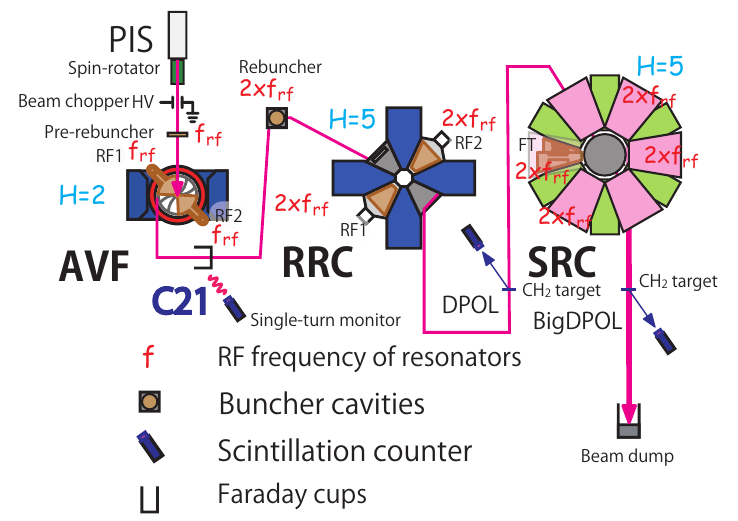
\includegraphics[width=\linewidth]{sakamoto2016_p1_fig1.png}
\caption{Acceleration and monitoring layout. Original crop: Sakamoto et al.\cite{Sakamoto2016}, PDF p. 1 / printed p. 145, Fig. 1. CC BY 3.0.}
\end{minipage}\hfill
\begin{minipage}[t]{0.47\linewidth}\centering
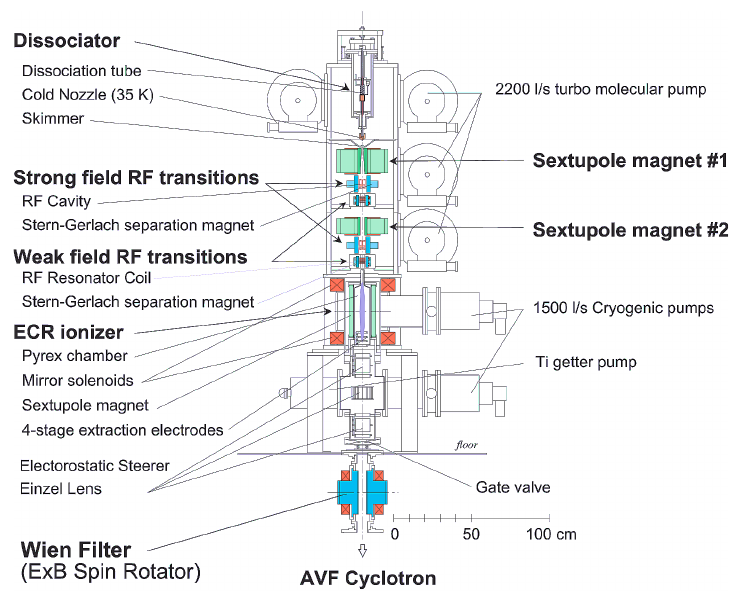
\includegraphics[width=\linewidth]{sakamoto2016_p1_fig2.png}
\caption{Polarized ion source. Original crop: Sakamoto et al.\cite{Sakamoto2016}, PDF p. 1 / printed p. 145, Fig. 2. CC BY 3.0.}
\end{minipage}
\end{figure}

Historical source settings include a nozzle temperature near $37\unit K$, dissociator RF power of $60$--$80\unit W$, and a $2.45\unit{GHz}$ ECR ionizer operating at roughly $30$--$40\unit W$. Current operation uses the facility's source settings and maintenance procedures.\src{Ikegami1993}{PDF p. 2 / printed p. 215}

\clearpage
\section{Spin populations, axis control and acceleration}
For populations $N_++N_0+N_-=1$ along the source symmetry axis $Z$,
\begin{equation}
P=N_+-N_-,\qquad T=1-3N_0,\qquad
N_\pm=\frac{2+T\pm3P}{6}.
\end{equation}
Here $P$ and $T$ denote vector and tensor polarization along that axis. Physical populations satisfy $-2\le T\le1$ and $3|P|\le2+T$.\src{Saito2026}{PDF p. 3, Sec. 2.1, Eq. (1)}
For an axially symmetric state with axis $\hat{\bm n}$,
\begin{equation}
\bm p=P\hat{\bm n},\qquad p_{ij}=\frac{T}{2}(3n_i n_j-\delta_{ij}).\label{eq:axial}
\end{equation}
RF transitions set $P,T$, while Wien-filter settings rotate $\hat{\bm n}$. Reversing the axis reverses the vector polarization and preserves the tensor. Positive and negative tensor modes are selected through their spin populations. The 2004 experiment included the ideal pure-tensor mode $(P,T)=(0,-2)$.\src{Sekiguchi2004}{arXiv PDF p. 5, Sec. II A}

\begin{figure}[H]\centering
\begin{minipage}[t]{0.43\linewidth}\centering
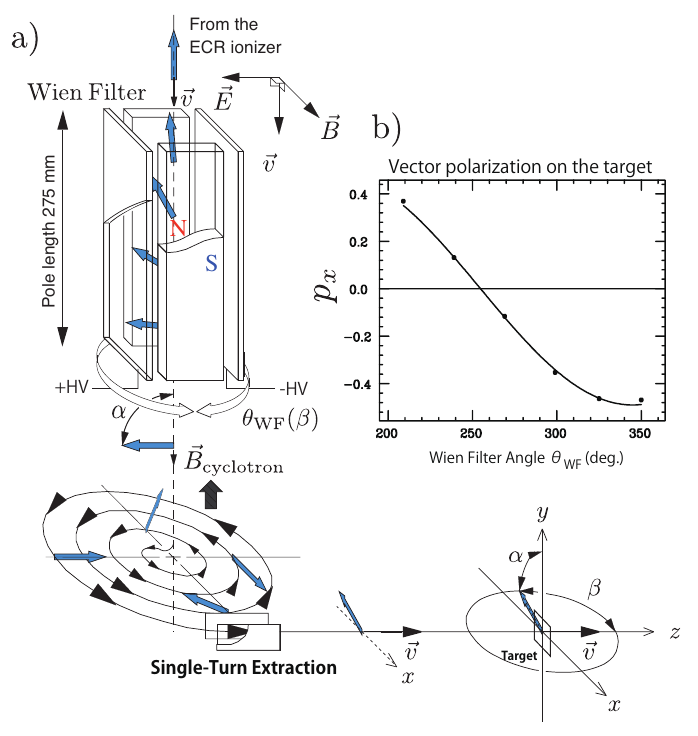
\includegraphics[width=0.9\linewidth]{sakamoto2016_p2_fig3.png}
\caption{Wien-filter axis calibration. Original: Ref.\cite{Sakamoto2016}, PDF p. 2 / printed p. 146, Fig. 3. CC BY 3.0.}
\end{minipage}\hfill
\begin{minipage}[t]{0.51\linewidth}\centering
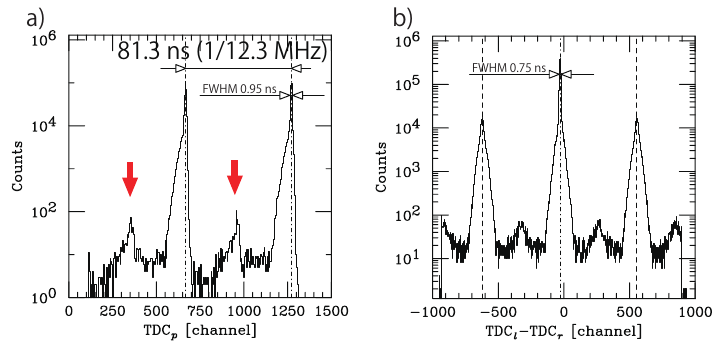
\includegraphics[width=\linewidth]{sakamoto2016_p3_fig6.png}
\caption{RF timing and coincidence spectra used for single-turn diagnostics. Original: Ref.\cite{Sakamoto2016}, PDF p. 3 / printed p. 147, Fig. 6. CC BY 3.0.}
\vspace{5pt}
\small\raggedright Single-turn extraction selects a common spin phase. The reported example had a turn-mixing fraction of $0.07\%$; stable operation over 2--3 days achieved purity above $99\%$.\src{Sakamoto2016}{PDF pp. 3--4}
\end{minipage}
\end{figure}

\textbf{Historical nominal 190 MeV/u recipe.} The following values come from Sakamoto et al., Table 2; the harmonic numbers appear in Table 1.\src{Sakamoto2016}{PDF p. 2 / printed p. 146}
\begin{center}\small
\begin{tabular}{lrrr}\toprule
Parameter & AVF & RRC & SRC \\\midrule
Output energy (MeV/u) & 4.0 & 70.4 & 187.5 \\
RF frequency (MHz) & 12.3 & 24.6 & 24.6 \\
Harmonic number & 2 & 5 & 5 \\
Extraction turn separation (mm) & 4.0 & 6.6 & 7.6 \\\bottomrule
\end{tabular}
\end{center}
Each operating period should retain the extraction settings, RF timing spectrum, turn-purity estimate and measured axis direction. Energy or extraction changes trigger a fresh polarization check.

\clearpage
\subsection*{RF transitions and reference data}
Okamura et al. connect the RF settings to the selected hyperfine states and measured source-axis polarization $P,T$. SX denotes a sextupole selector; SFT and WFT are strong- and weak-field transition units.\src{Okamura1995}{full APR PDF p. 179 / printed p. 148}

\shot{okamura1995_p179_table1.png}{0.46}{Historical RF-mode table with all footnotes. Source: Okamura et al.\cite{Okamura1995}, APR 28 PDF p. 179 / printed p. 148, Table 1. Blank measured components were not reported as zero.}{fig:rf-modes-en}

For ideal $(P,T)=(0,-2)$, WFT\#1 drives $1\to4$ and SFT\#2 drives $3\to5$, leaving states 2 and 5 at the ionizer; the measured $T$ was $-1.23$. Two routes to ideal $(0,+1)$ gave $T=+0.77$ and $+0.58$. Footnote b limits WFT\#2 power to below $0.4\unit W$ for the listed negative pure-vector mode to keep its tensor component negligible. Current modes require separate measurements.

\textbf{Intermediate-energy reference data.} Sekiguchi et al. give $A_y^d,A_{yy},A_{xx},A_{xz}$ at total energies $E_d=140,200,270\unit{MeV}$ (70/100/135 MeV/u). Their D-room and target-front Swinger instruments used left/right/up/down detector pairs.\src{Sekiguchi2002}{PDF p. 3, Sec. II B; pp. 9--12}

\begin{center}\small
\begin{tabularx}{\linewidth}{rrp{39mm}Y}\toprule
$E_d/2$ (MeV/u) & $E_d$ (MeV) & Tables / PDF pages & Reference use \\\midrule
70 & 140 & 2002: IV / 9; V / 10 & Upstream reference energy; V is D-room data.\\
100 & 200 & 2002: VI / 10 & January 2026 run energy.\\
135 & 270 & 2002: VII / 11; VIII / 12 & Historical measurements.\\
186.6 & 373.2 & 2017: I / 8, with cover & SRC high-energy data.\\\bottomrule
\end{tabularx}
\end{center}
The 2002 tables use Cartesian components and statistical errors; the 2017 table uses spherical components. Match the actual energy and acceptance to each dataset, including the distinction between 70 and 70.4 MeV/u. The Chinese edition reproduces Table V.\src{Sekiguchi2002}{PDF p. 7, Sec. III B}

\clearpage
\section{Reference polarimetry and recent operation}
\textbf{AVF / C-22, September 2024.} A $7\unit{MeV/u}$ beam was measured using $^{12}\mathrm C(\vec d,p)^{13}\mathrm C_{\rm g.s.}$ on a $0.5\unit{mg/cm^2}$ natural-carbon target. Two telescopes at $\theta_{\rm lab}=60^\circ$ used $0.5\unit{mm}$ plastic and $58\unit{mm}$ NaI(Tl). Four source modes, including an unpolarized reference, cycled every $5\unit s$.\src{Sugahara2025}{PDF p. 1 / printed p. 36, Table 1}

\shot{sugahara2025_p1_table2.png}{0.90}{Measured vector and tensor polarization in September 2024. Original crop: Sugahara et al.\cite{Sugahara2025}, PDF p. 1 / printed p. 36, Table 2. Mode labels and uncertainties follow the source.}{fig:modes}
The measured values provide a separate calibration for each source mode. An experimental beam specification should therefore state the required $P,T$, axis, mode sequence and tolerated residual vector component.

\textbf{AVF + RRC / D-room, January 2026.} Sugahara's EFB2026 report records a $100\unit{MeV/u}$ run on 9--16 January, about 150 hours, using $d$--$p$ elastic scattering in the D-room polarimeter. This supplies a recent operating reference for the source and intermediate-energy polarimetry.\src{SugaharaTalk2026}{PDF p. 4 / slide 3}

\shot{sugahara2026_p4_droom.png}{0.64}{D-room polarimeter shown in the 2026 report. Original crop: Sugahara\cite{SugaharaTalk2026}, PDF p. 4 / slide 3, upper-right photograph. The operating-condition table is on the same slide.}{fig:droom}

\textbf{Two-station precedent.} In the 2004 experiment, a D-room polarimeter measured the beam after RRC, while a Swinger polarimeter measured the target-bound beam before and after each run. The latter followed the beam-swinger motion, providing a direct check of the transported polarization.\src{Sekiguchi2004}{arXiv PDF p. 6, Sec. II B}

\clearpage
\section{Intermediate- and high-energy data and the absolute scale}
\textbf{BigDpol at 186.6 MeV/u.}
Sekiguchi et al. measured all deuteron analyzing powers with BigDpol at $186.6\unit{MeV/u}$. The SRC-extracted beam had an intensity of $4$--$8\unit{nA}$ and struck a $330\unit{mg/cm^2}$ CH$_2$ target. Four detector pairs identified elastic events through deuteron--proton coincidence; Dpol monitored the reference polarization at $70\unit{MeV/u}$. The $T_{21}$ measurement used a horizontal spin axis at $45.0^\circ\pm1.1^\circ$ to the beam.\src{Sekiguchi2017}{PDF pp. 3--4, Sec. II}

\shot{sekiguchi2017_p8_table1.png}{0.54}{Experimental analyzing powers at 186.6 MeV/u, with statistical uncertainties. Original: Sekiguchi et al.\cite{Sekiguchi2017}, \textbf{CHORUS PDF p. 8 / manuscript p. 7, Table I}. The cover counts as PDF p. 1.}{fig:ap}

The absolute calibration uses
\[
{}^{12}\mathrm C(\vec d,\alpha){}^{10}\mathrm B^*[2^+],\qquad
A_{yy}(0^\circ)=-\frac12,
\]
with the analyzing power fixed by parity. This calibrates the $d$--$p$ reference response used in routine beam measurements.\src{Sekiguchi2004}{arXiv PDF p. 6, Sec. II B}\cite{Suda2007}

For each dataset, retain its beam energy, angular convention, interpolation range and uncertainty model. The 2017 paper reports a beam-polarization uncertainty below $4\%$ in addition to the statistical errors in Table I. Shared calibration errors remain correlated between polarimeters.\src{Sekiguchi2017}{PDF p. 4, end of Sec. II}

\clearpage
\section{From detector yields to the target spin state}
\textbf{Polarization extraction.} Let local $z$ follow the beam and $+y$ be the left-arm scattering normal. For an axial state along $y$ and an unpolarized target, the Cartesian convention gives
\begin{equation}
\sigma_{L,R}=\sigma_0\left(1\pm\frac32 PA_y+\frac12 TA_{yy}\right).
\end{equation}
For polarized-to-unpolarized yield ratios $r_L,r_R$, corrected for luminosity, efficiency and live time,
\begin{equation}
P=\frac{r_L-r_R}{3A_y},\qquad T=\frac{r_L+r_R-2}{A_{yy}}.
\end{equation}
The difference determines the vector term; the common yield change determines the tensor term. For finite acceptance, use the weighted response
\begin{equation}
A^{\rm eff}_{k,a}=\frac{\int dE\,d\Omega\;w_a\sigma_0 A_k}
{\int dE\,d\Omega\;w_a\sigma_0},
\end{equation}
where $w_a$ includes geometry, efficiency, target energy loss and event selection. Cartesian and spherical analyzing powers must share a defined coordinate conversion. These expressions summarize the measurement model used in this note.

\textbf{Spin transport.} Magnetic-dipole transport produces a rotation $R$ along each trajectory:
\begin{equation}
\rho'=U(R)\rho U^\dagger(R),\quad \bm p'=R\bm p,\quad Q'=RQR^{\mathsf T},\qquad Q_{ij}=p_{ij}.
\end{equation}
A common rotation preserves the tensor eigenvalues. A distribution of rotations changes the measured ensemble average, with weights set by the accepted beam phase space. Integrate the orbit and BMT spin equation through the actual magnet sequence, including the field traversed before the reaction vertex.\cite{BMT1959}

For an ideal transverse dipole and an initially longitudinal tensor axis,
\begin{equation}
\psi=G_d\gamma\theta,\qquad \gamma=1+\frac{K_d}{m_dc^2},\qquad
\frac{p_{zz}^{\rm out}}{T}=\frac{3\cos^2\psi-1}{2}.
\end{equation}
Here $\psi$ is the spin angle relative to momentum. At nominal $190\unit{MeV/u}$, $K_d=380\unit{MeV}$ and CODATA 2022 gives $G_d\gamma=-0.17195655$. An illustrative $30^\circ$ bend gives $\psi=-5.1587^\circ$ and the longitudinal tensor projection $p_{zz}^{\rm out}/T=0.987873$.\cite{CODATA2022}

The SAMURAI calculation should use current magnet settings, field maps, beam energy, apertures and target position. The official BigRIPS optics page provides reference orbit maps for the SAMURAI beam line. Two polarimeters can test a specified transport model through their predicted detector yields. For an axial source model, the fitted state is $P,T,\hat{\bm n}$; a general spin-1 state has eight real polarization components.\src{BigRIPSOptics}{SAMURAI Beam Line entries}

\textbf{Measured axis verification at RIKEN.} After their main experiment, Mardanpour et al. rotated the SMART swinger dipole by $90^\circ$ in a vertical plane and used two polarimeters before and after spin precession. At total energies 130/180 MeV (65/90 MeV/u), the measured polar axis angles were $\beta=82.0^\circ\pm0.5^\circ$ and $99.4^\circ\pm0.5^\circ$; both azimuthal angles were $\alpha=2.0^\circ\pm0.5^\circ$. These are axis directions, distinct from $\psi$.\src{Mardanpour2007}{arXiv v2 PDF p. 5}

The $T_{21}$ response contains $\sin\beta\cos\beta$, so an axis near $90^\circ$ weakens sensitivity and increases the uncertainty from its direction. For SAMURAI, a horizontal or longitudinal source state and both stations' azimuthal responses can test the predicted rotation; propagate the measured axis uncertainty to the target.\src{Mardanpour2007}{PDF pp. 2, 5, Eq. (1)}

\clearpage
\section{Role of Sekiguchi's team during beam time}
The practical role to discuss with Sekiguchi's team is \textbf{setting up the polarized beam and maintaining a measured spin state during data taking}. Their laboratory reports PIS preparation and beam tests. The operating roles below are inferred from that work and the published beam procedures; personnel and control-room assignments are agreed for each experiment.\src{SekiguchiLab2025}{PDF p. 1 / printed p. 370, Research Activity}

\textbf{1. Tune the PIS polarization modes with the source specialists.}
Select the required RF-transition modes, measure $P,T$ for each mode after AVF, and use those measurements to optimize the transition settings. Check the beam current and stability alongside polarization. The 2024 recovery test provides a concrete example: three polarized modes were measured and further optimization was planned for mode 3.\src{Sugahara2025}{PDF p. 1, Table 2 and following paragraph}

\textbf{2. Set and verify the spin direction.}
Set the Wien-filter field and rotation angle for the requested vertical, horizontal or longitudinal axis. Scan the settings and use polarimeter asymmetries to identify the required orientation after acceleration. Repeat the axis check after a change in energy or extraction conditions.\src{Sakamoto2016}{PDF p. 2, Fig. 3}\src{Sekiguchi2017}{PDF p. 4, Sec. II}

\textbf{3. Check single-turn extraction jointly with the accelerator crew.}
Use the AVF chopper monitor and downstream beam--RF timing spectra to identify satellite bunches and estimate turn mixing. At SRC, BigDpol measures recoil-proton timing relative to an RF reference at $f_{\rm beam}/2$. Feed the timing results back to the crew tuning phase acceptance, flat-top RF and extraction. RIKEN assigns cyclotron and polarized-deuteron single-turn operation to Sakamoto's Cyclotron Team.\src{Sakamoto2016}{PDF p. 3, Figs. 4--6}\src{CyclotronTeam}{Research Summary, items 2, 3 and 6}

\textbf{4. Operate the polarimeters and determine the beam polarization.}
Set up the target and detector pairs, establish elastic-scattering coincidence gates, collect polarized and unpolarized yields, and apply calibrated analyzing powers. Provide $P,T$, the axis and uncertainties after tuning. The 2017 experiment continuously monitored the reference beam with Dpol at $70\unit{MeV/u}$.\src{Sekiguchi2017}{PDF pp. 3--4, Sec. II}

\textbf{5. Run the mode sequence and watch polarization during data taking.}
Cycle the agreed source modes, synchronize the mode labels with DAQ, and track polarization, beam normalization, live time and RF timing. Accumulate enough cycles for the required precision. The published experiments used a five-second mode cycle; the 2004 Swinger measurements checked the target-bound beam before and after each run.\src{Sekiguchi2017}{PDF p. 4}\src{Sekiguchi2004}{arXiv PDF pp. 5--6}

\textbf{6. Diagnose changes and qualify the beam after recovery.}
When polarization changes, compare the source modes, timing spectra and upstream/downstream polarimeter responses. Use that evidence to choose the next action with the source or accelerator specialists, then remeasure the polarization and axis after recovery. For SAMURAI, agree who performs the final check from the last polarimeter to the reaction target.

For planning, assign an operator and backup to each of these six activities. The key discussion with Sekiguchi's team is which PIS/Wien adjustments and polarimeter shifts they would perform, which timing diagnostics they would analyze, and how they would coordinate retuning with the accelerator crew.

\clearpage
\section*{Sources and reproduction}
The eight original source crops use PDF page numbers counted from the first page, including covers. \texttt{sources.json} records URLs, SHA-256 hashes and crop coordinates; the Chinese edition gives the extended index. Sources were checked on 7 September 2026, following the \href{https://chatgpt.com/share/6a9e507f-ba88-83ee-930f-861c5ef504c1}{shared research discussion}.

From the repository root, run \texttt{make -C docs/polarization\_production\_transport en}; replace \texttt{en} with \texttt{verify} to check source PDFs and crops.

\begingroup\footnotesize
\linespread{1.0}\selectfont
\setlength{\bibsep}{0pt}
\bibliographystyle{unsrtnat}
\bibliography{references_en}
\endgroup
\end{document}
